\documentclass[12pt]{article}

% Some typesetting decisions
\usepackage[utf8]{inputenc}

% Typesetting and basic formatting. 
% This PDF is made to be read on-screen,
% so we use large fonts and little margin
\usepackage[margin=30mm]{geometry}
\usepackage{fourier}
\usepackage{setspace}
\usepackage{graphicx}
\setstretch{1.1}
\setlength{\parindent}{0pt}
\setlength{\parskip}{12pt}
\frenchspacing
\sloppy


% Links
\usepackage{xcolor}
\usepackage{hyperref}
\hypersetup{colorlinks,linkcolor={green!50!black},citecolor={blue!50!black}, urlcolor={red!50!black}}  
% This one is for demo-purposes only, don't use it in your submission ;) 
\usepackage{blindtext}

% Citation with natbib: 
% Use \citet{} and \citep{} only, not \cite{}
\usepackage{natbib}
\bibliographystyle{abbrvnat}



% Custom (maths) commands
\usepackage{amsmath, amssymb}
\usepackage{bm}

\newcommand{\Ebb}{\mathbb{E}}
\newcommand{\Rbb}{\mathbb{R}}
\newcommand{\Sbb}{{\mathbb{S}}}
\newcommand{\Tbb}{\mathbb{T}}
\newcommand{\Nbb}{\mathbb{N}}
\newcommand{\Xbb}{{\mathbb{X}}}
\newcommand{\Pbb}{\mathbb{P}}
\newcommand{\Dbb}{\mathbb{D}}
\newcommand{\Ybb}{\mathbb{Y}}
\newcommand{\onebb}{\mathbb{1}}
\newcommand{\Ncal}{\mathcal{N}}
\newcommand{\Mcal}{\mathcal{M}}
\newcommand{\Lcal}{\mathcal{L}}
\newcommand{\Bcal}{\mathcal{B}} 
\newcommand{\Qcal}{\mathcal{Q}} 
\newcommand{\Acal}{\mathcal{A}}
\newcommand{\Xcal}{\mathcal{X}}
\newcommand{\Tcal}{\mathcal{T}}
\newcommand{\Pcal}{\mathcal{P}}
\newcommand{\Zcal}{\mathcal{Z}}
\newcommand{\Rcal}{\mathcal{R}}
\newcommand{\Ocal}{\mathcal{O}}
\newcommand{\Fcal}{\mathcal{F}}
\newcommand{\Dcal}{\mathcal{D}}
\newcommand{\Ycal}{\mathcal{Y}}
\newcommand{\Ecal}{\mathcal{E}}
\newcommand{\Hcal}{\mathcal{H}}
\newcommand{\Ucal}{\mathcal{U}}
\newcommand{\Ccal}{\mathcal{C}}
\newcommand{\Ical}{\mathcal{I}}
\newcommand{\diff}{\,\text{d}}
\DeclareMathOperator{\diag}{diag}
\DeclareMathOperator{\cond}{cond}
\DeclareMathOperator{\gp}{GP}
\DeclareMathOperator{\divergence}{div}
\DeclareMathOperator{\curl}{curl}
\DeclareMathOperator{\supp}{supp}
\DeclareMathOperator*{\argmax}{arg\,max}
\DeclareMathOperator*{\argmin}{arg\,min}






% Insert the title of your presentation, your name, and your e-mail here.
% Leave the rest as is.
\title{\vskip-3em \bf 
	Simulation-based Inference
    }
\author{
    A Summary Written by Stefan Wezel \\
    \texttt{stefan.wezel@student.uni-tuebingen.de}
}
\date{\it Machine Learning for and with Dynamical Systems\\Summer Term 2021}


\begin{document}

\maketitle

\begin{abstract}\vskip-1.5em \noindent
Simulators are used across different scientific domains where serve as valuable tools to encode empirical knowledge about a system of interest. Inference in this setting often boils down to finding parameters of the simulator for a given, real-world observation, which typically cannot be computed analytically.\citet{papamakarios2016fast} propose to learn a posterior over a simulators parameters by using neural density estimators. Here, we give an overview of their work and SBI in general.
\end{abstract}


\section*{Problem Setting and Related Work}
Scientific fields, such as population genetics, particle physics, epidemiology, astrophysics among others make use of sophisticated simulators to model observed systems \citep{brehmer2020simulation, de2020simulation, delaunoy2020lightning,cranmer2020frontier, pritchard1999population}. These simulators are able to encode prior knowledge like causal relations, hierarchies of variables, ... Performing inference in this setting, however, would require a finding a posterior over parameters $\theta$ for a given observation $x_0$. This can be stated in closed form as 
\begin{align}
	p(\theta|x=x_0) = \frac{p(x|\theta)p(\theta)}{p(x)} = \frac{\overbrace{\int p(x,z|\theta)dz}^{intractable} p(\theta)}{\underbrace{\int p(x|\theta)p(\theta)d\theta}_{intractable}},
\end{align}
where $z$ is a nuisance parameter. If likelihood and evidence are intractable, which is typically the case, this cannot be computed analytically. Intuitively, it can be thought of as inverting the simulator.\\
A collective term for methods to solve this inverse problem is Approximate Bayesian Computation (ABC). The most simple approach is rejection ABC \citep{pritchard1999population} where samples produced by a simulator are discarded if notis within a $\epsilon$-ball around the observation of interest. For small values of $\epsilon$ this method may take many steps to even produce a single matching parameter set. For large $\epsilon$ it is not precise. Moreover, this method does not produce a full posterior over the parameter but merely yields point estimates with confident intervals. With Markov-Chain-Monte-Carlo ABC and Sequential ABC improvements over rejection ABC have been proposed. These methods produce samples more efficiently. While this can lead to faster convergence, it does not produce a full posterior over parameters that is conditioned on the actual observation, but rather a sample that is close to it.

%In practice these resulting pseudo-distributions are often much wider than the actual posterior. [citation needed]
 



\section*{Neural Approach}
\citet{papamakarios2016fast} build on recent advances in deep learning to learn a posterior over parameters directly from sample produced by a simulator. They use Deep Neural Networks (DNN) to parameterize a Gaussian Mixture Model (GMM). They use the simulator to perform $n$ simulations and storing pairs of samples $x$ and corresponding parameters $\theta$. This gives the set $\lbrace(x_i,\theta_i)\rbrace_{i \in n}$ which they use as training data. DNNs are fitted to parameterize a GMM

\begin{align}
	\sum_k \alpha_k \mathcal{N}(\theta|m_k, S_k) = \sum_k f_1(x)_k \mathcal{N}(\theta|f_2(x)_k, diag(f_3(x))_k)
\end{align}
, where $k$ is the number of components, $m$ the mean and $S$ the covariance matrix of a Gaussian, and $f_{\lbrace 1,2,3 \rbrace}$ are MLPs.


\begin{figure}
	\centering
	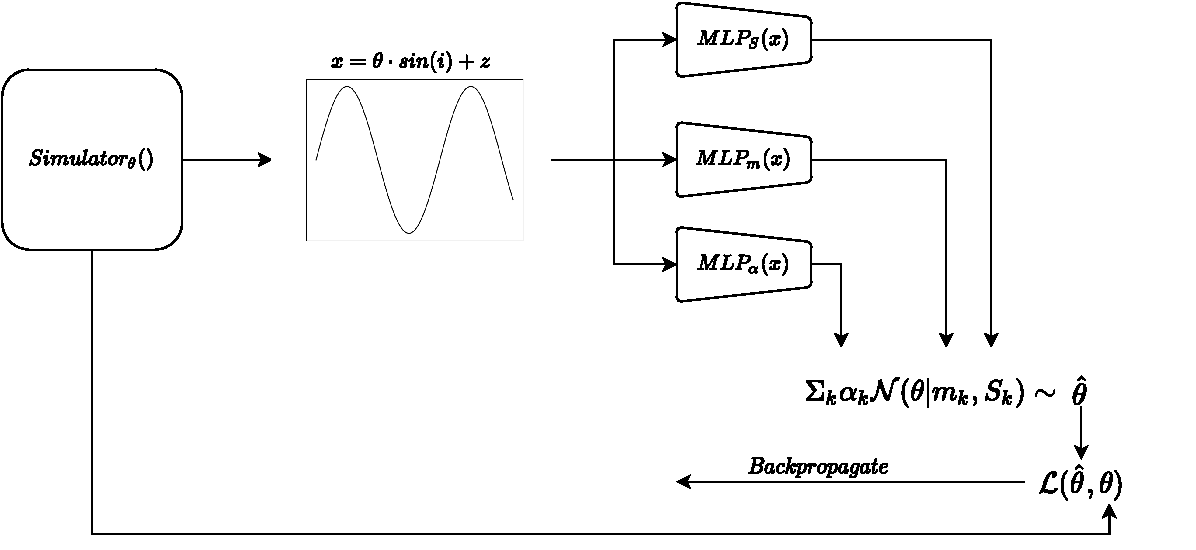
\includegraphics[width=.8\linewidth]{figures/sbi_vis.pdf}
	\caption{Given samples by the simulator, Multilayer perceptrons (MLP) are trained to parameterize a distribution over parameters generating the sample. A training signal is created by sampling from this distribution and comparing the sample to the actual parameters which are known.}
%	\label{fig:fhave}
\end{figure} 

\section*{Possible Enhancements/Open Ends}
\section*{Conclusion}







Use only the provided maths commands use \texttt{align} for embedded maths (not \texttt{align*}):
\begin{align}
    \Fcal, \Rbb, \Nbb
\end{align}
The \texttt{diff} command is for proper typesetting in integrals: $\int f(x) \diff x$, not $\int f(x) dx$.
If you need conditional probabilities, use \texttt{mid} for $A$ conditioned on $B$: $p(A \mid B)$.

Write clearly; pay attention to clarity, simplicity, and -- above all -- correctness of your statements. Look up how to write a scientific document.

\bibliography{references}
\end{document}